\subsection{Dataset}
	%%%%%%%%%%%%%%%%%%%%%%%%%%%%%%%%%%%%%%%%%%%%%%%%%%%%%
	In this work, we have generated a large dataset of 475 cases of a full wavefield of propagating Lamb waves in a plate made of carbon fibre-reinforced plastic (CFRP).
	The time-domain spectral element method was used for simulation of Lamb wave interaction with delamination~\cite{Kudela2020}.
	For each case, single delamination was modelled by using the method of splitting nodes between appropriate spectral elements. 
	It was assumed that the composite laminate is made of eight layers of a total thickness of 3.9 mm.
	The delamination was modelled between the third and fourth layer (see Fig.~\ref{fig:plate_setup} for details).
	It should be noted that the figure shows an exaggerated cross-section through the delamination. 
	Zero-volume delamination was assumed in the model. 
	For each case delamination location was selected randomly so that interaction of guided waves excited at the plate centre with delamination is different for each case.
	It includes cases when delamination is located at the edge of the plate which is the most difficult to identify by signal processing methods.
	Additionally, the size of the delamination was randomly simulated by selecting the ellipse minor and major axis from the interval 10--40 mm.
	Also, the angle between the delamination major axis and the horizontal axis was randomly selected.
	\begin{figure}
		\centering
		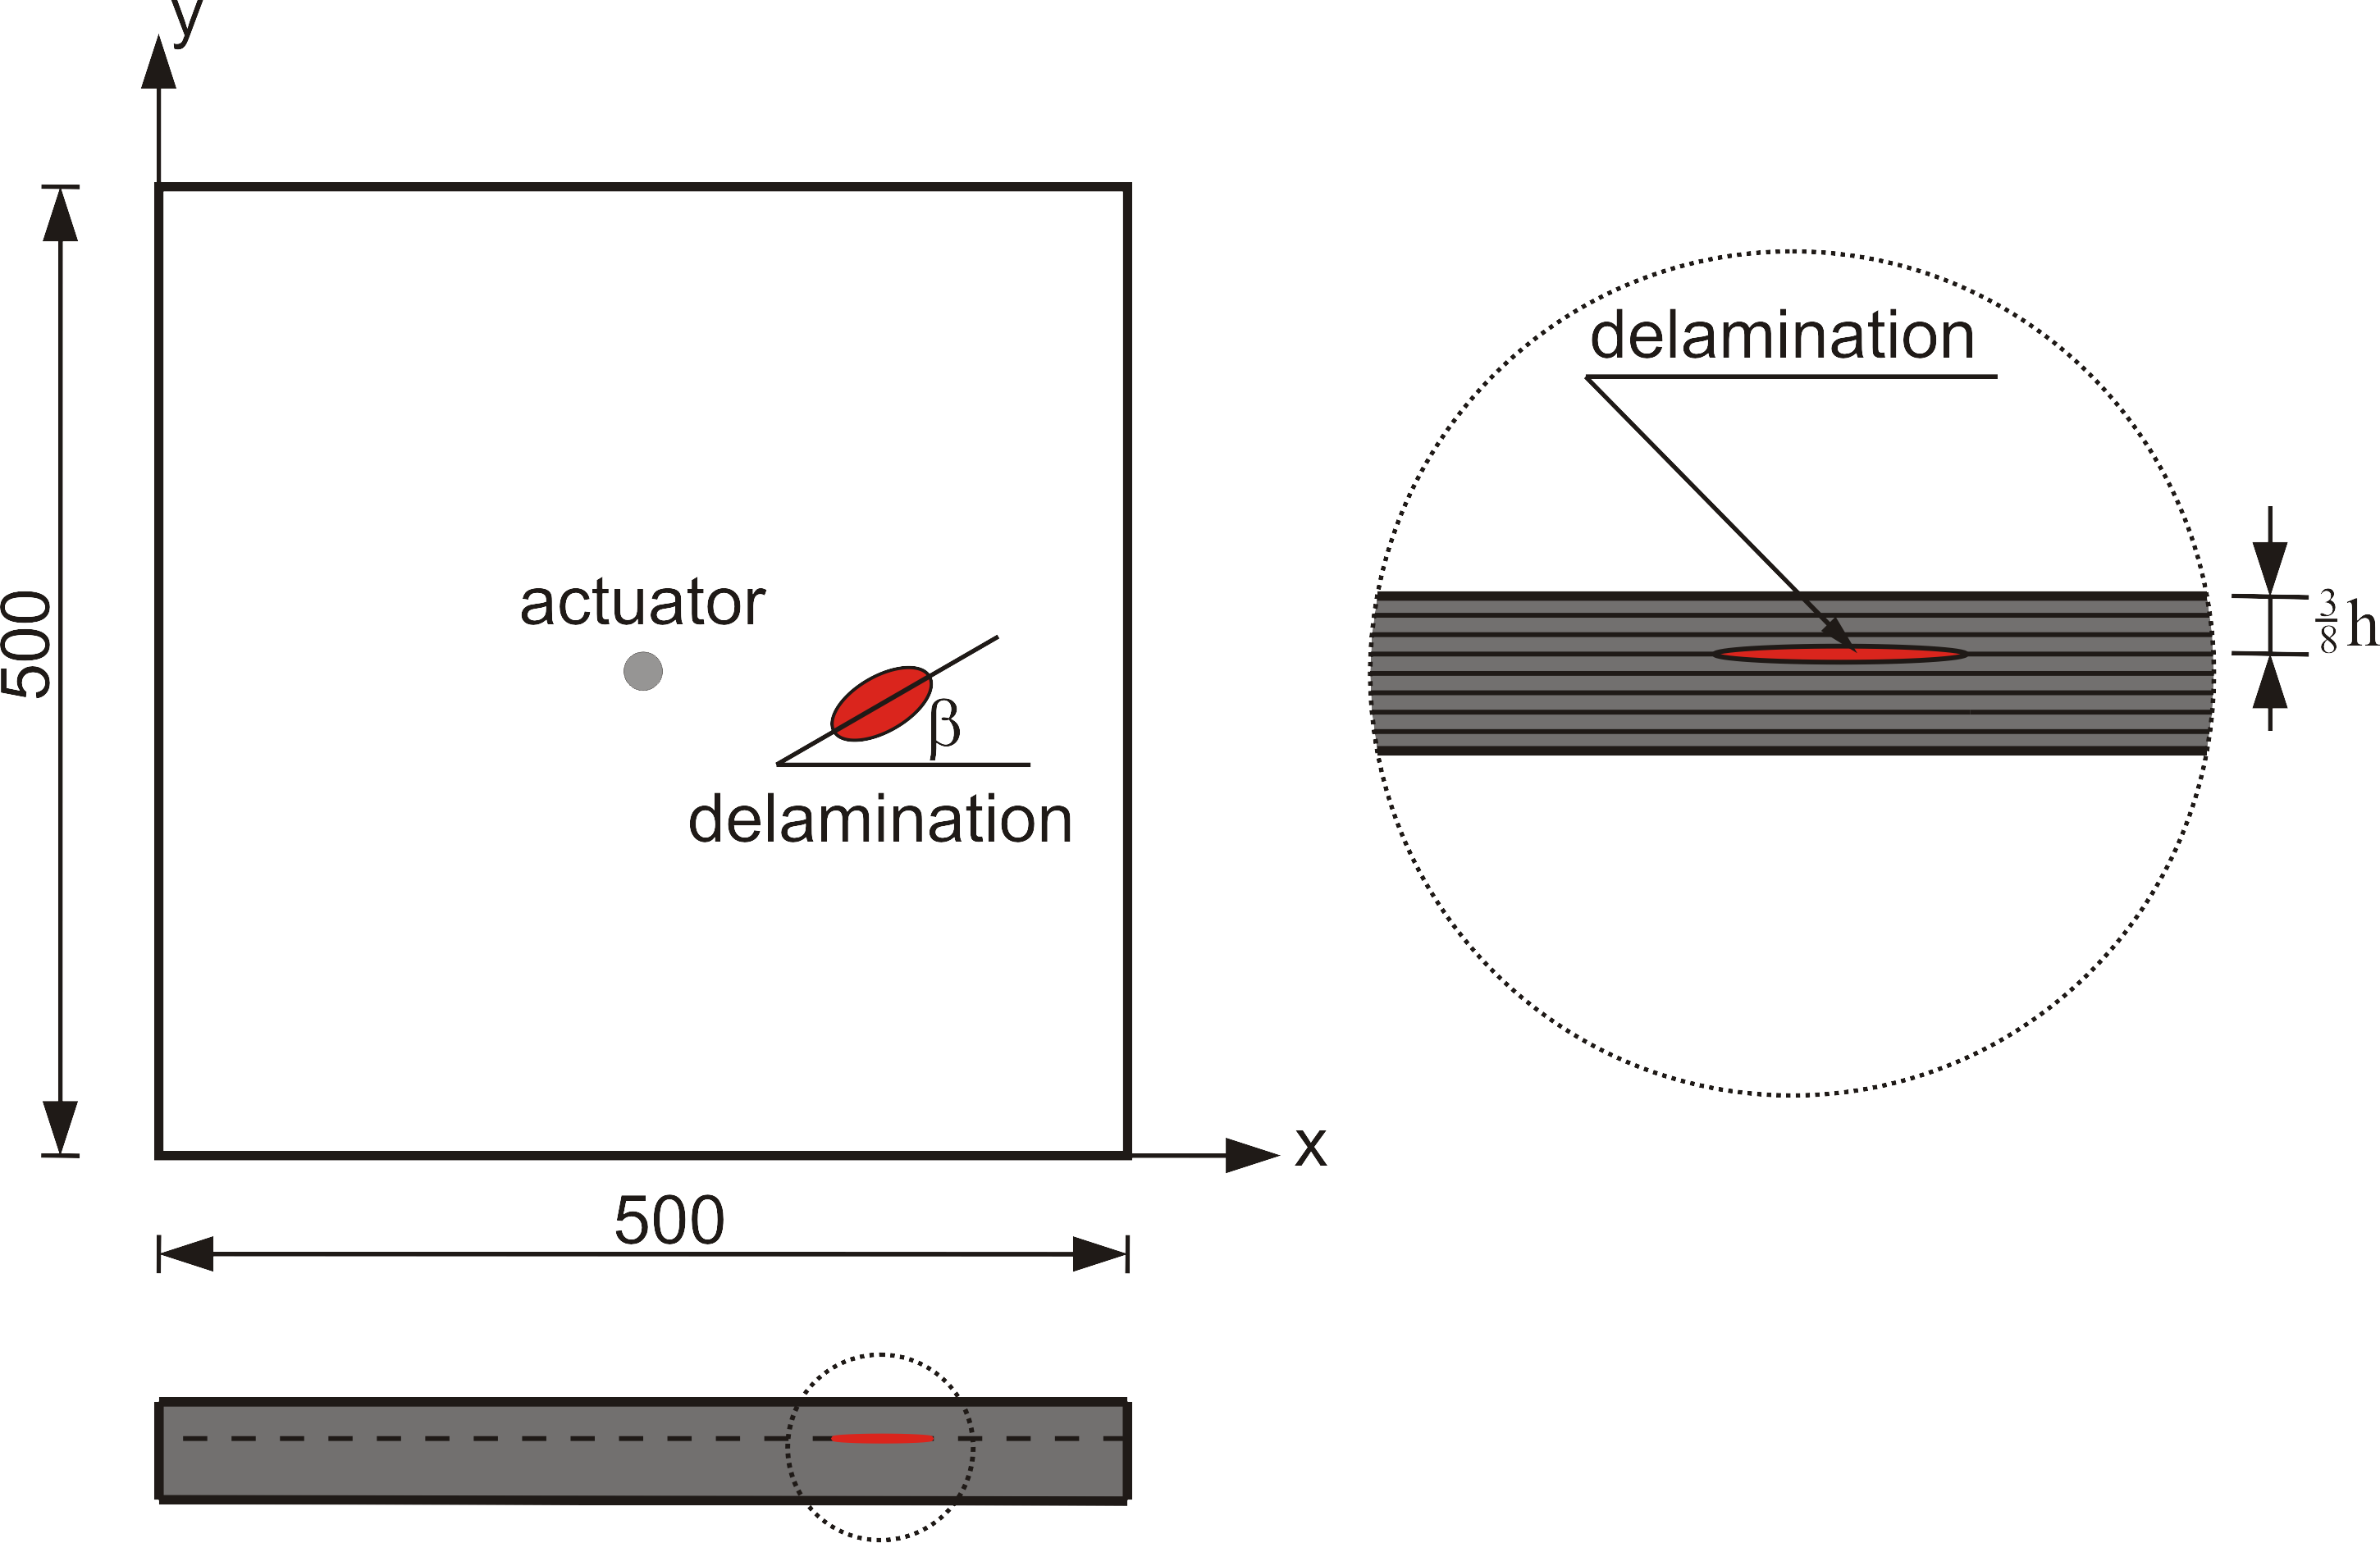
\includegraphics[scale=0.8]{plate_delam_arrangement_MSSP.png}
		\caption{Setup for computing Lamb wave interactions with delamination.}
		\label{fig:plate_setup}
	\end{figure}

	The output from the top and bottom surface of the plate in the form of particle velocities at the nodes of spectral elements were projected on the uniform grid of 500\(\times\)500 points by using shape functions of elements (see Parallel spectral element method for guided wave based structural health monitoring paper for detail).
	It essentially resembles measurements acquired by SLDV in the transverse direction (perpendicular to the plate surface).
